% Szglab4
% ===========================================================================
%
\chapter{Szkeleton tervezése}

\thispagestyle{fancy}

\section{A szkeleton modell valóságos use-case-ei}
\comment{A szkeletonnak, mint önálló programnak a működésével kapcsolatos use-case-ek.}

\subsection{Use-case diagram}

\begin{figure}[h]
\begin{center}
%\includegraphics[width=17cm]{chapters/chapter05/example.pdf}
\caption{x}
\label{fig:SzkeletonUseCase}
\end{center}
\end{figure}

\subsection{Use-case leírások}
\comment{Minden use-case-hez külön}

\usecase{...}{...}{...}{...}

\pagebreak
\setlength\parindent{15mm}
\section{A szkeleton kezelői felületének terve, dialógusok}
A szkeleton menüvezérelt módon fog működni. A felhasználónak meg kell adnia a kívánt parancsnak a kódját, majd a program lefuttatja azt. A menü felépítése itt látható: \\
\begingroup 
\fontsize{10pt}{10pt}\selectfont
\texttt{
1. Torony építés \\
\indent *1.1 Érvényes helyre akarunk építeni? I\textbackslash N \\
\indent *1.2 Ütközik másik toronnyal? I\textbackslash N \\
2. Akadály építés \\
\indent *2.1 Érvényes helyre akarunk építeni? I\textbackslash N \\
\indent *2.2 Ütközik másik akadállyal? I\textbackslash N \\
3. Következő ellenség lekérése \\
\indent *3.1 Van következő ellenség? I\textbackslash N \\
4. Ellenség mozgatás \\
\indent *4.1 Elérte az ellenség a Waypointot? I\textbackslash N \\
\indent *4.2 Hatósugarában van egy akadálynak? I\textbackslash N \\
\indent \indent *4.2.1 Az akadályok van varázskő? I\textbackslash N \\
5. Torony tüzelés \\
\indent *5.1 Van a torony hatósugarán belül ellenség? I\textbackslash N \\
\indent \indent *5.1.1 Van a tornyon varázskő? I\textbackslash N \\
6. Lövedék mozgatása \\
\indent *6.1 Elérte az ellenséget? I\textbackslash N \\
7. Varázskő felrakása \\
\indent *7.1 Toronyra vagy akadályra? T\textbackslash A \\
8. Kilépés \\
} \\
\endgroup
A *-gal jelölt menüpontokat nem lehet kiválasztani, ezt a program automatikusan megteszi, ha a felhasználó a parancs szülőjét meghívta. Ezek (1 kivétellel) igen/nem típusú kérdések. A kérdések végén láthatóak a lehetséges válaszok.
\\
Az alábbi példa egy olyan interakciót mutat be, ahol a felhasználó építeni akar egy tornyot, ami érvényes helyen van, de ütközne egy másik toronnyal: \\
\begingroup
\fontsize{10pt}{10pt}\selectfont
\texttt{
? Adja meg a parancs kódját: 1 \\
- 1. Torony építése \\
>\indent ->[:Game].buildTower(pos): \\
>\indent \indent ->[:Map].canBuildTower(pos): \\
>\indent \indent \indent ->[:Waypoint].getPosition(): \\
?\indent \indent \indent 2.1. Érvényes a hely? I\textbackslash N: I \\
<\indent \indent \indent <-[:Waypoint].getPosition() \\
<\indent \indent <-[:Map].canBuildTower(): \\
>\indent \indent ->[:Game].collidesWithTower(pos): \\
>\indent \indent \indent ->[:Tower].getPosition(): \\
?\indent \indent \indent 2.2. Ütközik másik toronnyal? I\textbackslash N: I \\
<\indent \indent \indent <-[:Tower].getPosition() \\
>\indent \indent <-[:Game].collidesWithTower(pos) \\
>\indent <-[:Game].buildTower() \\
? Adja meg a parancs kódját:
} \\
\endgroup
Minden sor elején van 1 karakter, ami a sor típusát jelöli.
\begin{itemize}
\item '?': kérdés, felhasználói interakcióra vár
\item '-': megjegyzés
\item '>': metódusba lépés
\item '<': metódusból visszatérés
\end{itemize}
A metódusba lépéskor és visszatérésnél, egy nyíl jelöli, hogy hívásról vagy visszatérésról van-e szó majd szögletes zárójelek között található az objektumtípusa, ezután pedig a metódus neve. Például: ->[:Osztály].metódus():

\section{Szekvencia diagramok a belső működésre}
\comment{A szkeletonban implementált szekvenciadiagramok. Tipikusan egy use-case egy diagram. Ezek megegyezhetnek a korábban specifikált diagramokkal, de az egyes életvonalakat (lifeline) egyértelműen a szkeletonban példányosított objektumokhoz kell tudni kötni. Azt kell megjeleníteni, hogy a szkeletonban létrehozott objektumok egymással hogyan fognak kommunikálni.}

\section{Kommunikációs diagramok}
%\comment{A szkeletonban, az egyes szkeleton-use-case-ek futása során létrehozott objektumok és kapcsolataik bemutatására szolgáló %diagramok. Ezek alapján valósítják meg a szkeleton fejlesztői az inicializáló kódrészleteket.}

\begin{figure}[H]
\begin{center}
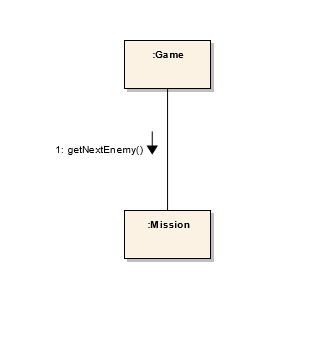
\includegraphics{images/ch05/nextEnemyKomm.png}
\caption{Ellenségek ütemezése.}
\label{fig:nextEnemyKomm}
\end{center}
\end{figure}

\begin{figure}[H]
\begin{center}
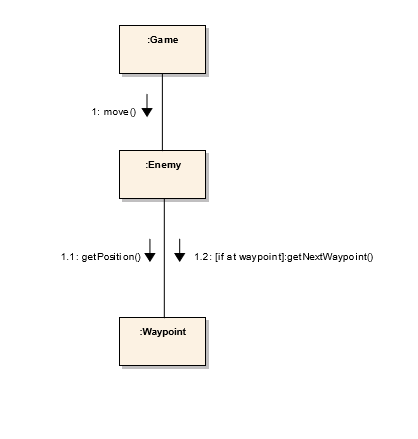
\includegraphics{images/ch05/moveKomm.png}
\caption{Ellenség mozgatása.}
\label{fig:moveKomm}
\end{center}
\end{figure}

\begin{figure}[H]
\begin{center}
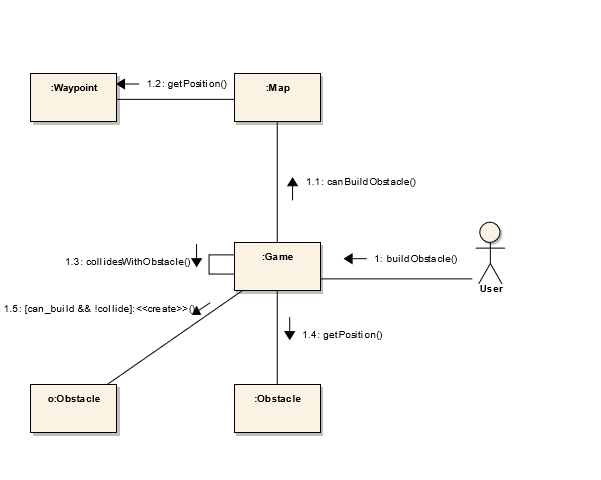
\includegraphics{images/ch05/buildObKomm.png}
\caption{Akadály építése.}
\label{fig:buildObKomm}
\end{center}
\end{figure}

\begin{figure}[H]
\begin{center}
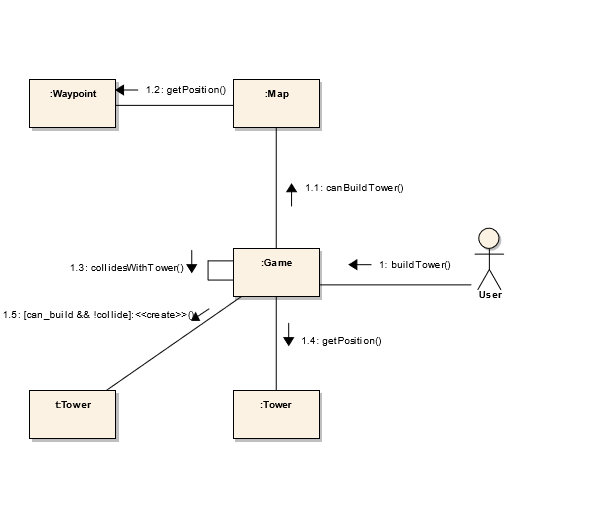
\includegraphics{images/ch05/buildTowerKomm.png}
\caption{Torony építése.}
\label{fig:buildTowerKomm}
\end{center}
\end{figure}

\begin{figure}[H]
\begin{center}
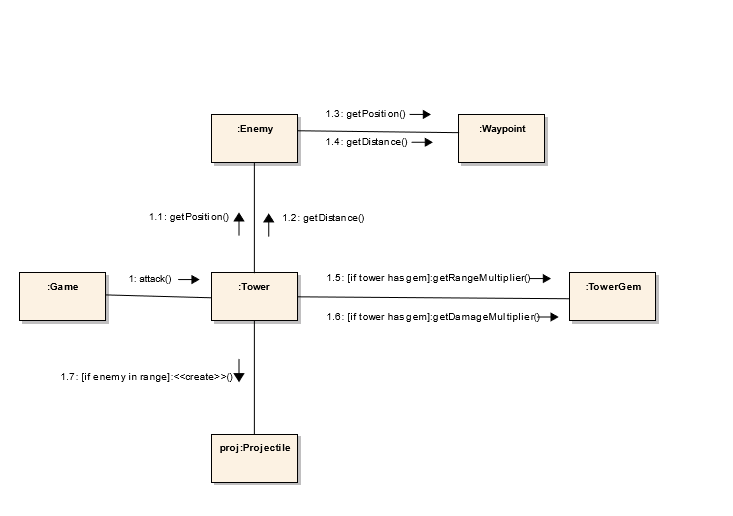
\includegraphics{images/ch05/attackKomm.png}
\caption{Torony tüzelése egy ellenségre.}
\label{fig:attackKomm}
\end{center}
\end{figure}

\begin{figure}[H]
\begin{center}
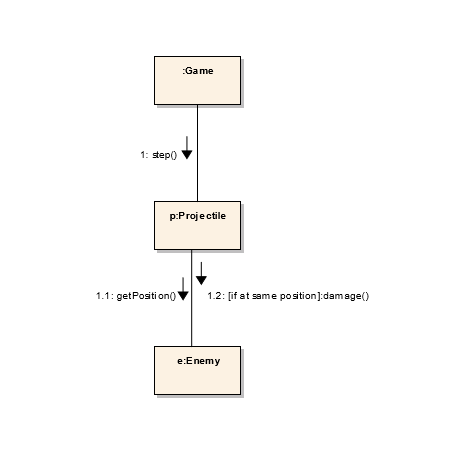
\includegraphics{images/ch05/projectileMoveKomm.png}
\caption{Lövedék mozgatása.}
\label{fig:projectileMoveKomm}
\end{center}
\end{figure}

\begin{figure}[H]
\begin{center}
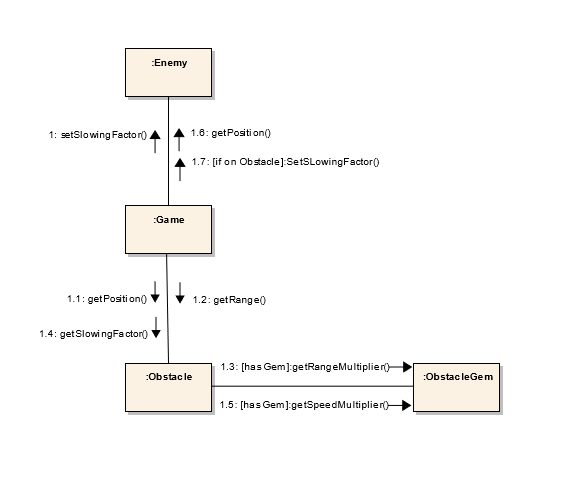
\includegraphics{images/ch05/slowKomm.png}
\caption{Akadályon áthaladó ellenség lassítása.}
\label{fig:slowKomm}
\end{center}
\end{figure}

\begin{figure}[H]
\begin{center}
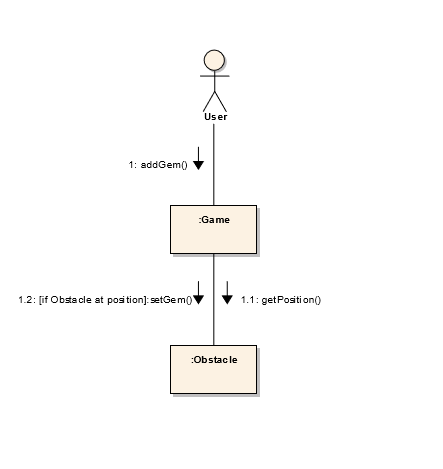
\includegraphics{images/ch05/addGemToObKomm.png}
\caption{Varázskő feltétele akadályra.}
\label{fig:addGemToObKomm}
\end{center}
\end{figure}


\begin{figure}[H]
\begin{center}
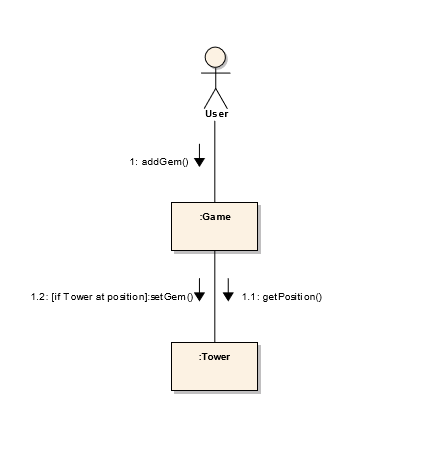
\includegraphics{images/ch05/addGemToTowerKomm.png}
\caption{Varázskő feltétele toronyra.}
\label{fig:addGemToTowerKomm}
\end{center}
\end{figure}